% Chapter 3 — Dataset Audit, Physical Coupling Analysis, and Experimental Protocol

This chapter documents the empirical foundation of the thesis: the complete audit of the 30 numerical Large Eddy Simulation (LES) operating conditions from the \textit{RealPDEBench} combustion benchmark~\cite{hu2026realpdebench}, the geometric and physical conventions of the two-dimensional diametral plane, the quantitative analysis of kinematic--thermal coupling and cross-condition ambiguity, and the leakage-free operating-condition split and decomposed evaluation protocol locked prior to model training. All figures and statistics reported in this chapter are computed directly from the staged simulation archive and training-only manifests without invoking any predictive reconstruction model.

% ==============================================================================
\section{The RealPDEBench Swirl-Combustor LES Dataset}
\label{sec:data_overview}
% ==============================================================================

\subsection{Numerical Simulation Configuration and Parameter Space}
\label{subsec:data_sim_config}

The numerical dataset originates from the combustion scenario of \textit{RealPDEBench}~\cite{hu2026realpdebench} (\texttt{AI4Science-WestlakeU/RealPDEBench}, Hub format \texttt{lazy\_slicing\_v2}, data version 2.0.1), simulating a swirl-stabilized $\text{NH}_3/\text{CH}_4/\text{air}$ co-firing gas-turbine model combustor. Three-dimensional unsteady Large Eddy Simulations (LES) were conducted with finite-rate chemical kinetics governed by a reduced mechanism comprising $38$ chemical species and $184$ elementary reactions, coupled with the Eddy Dissipation Concept (EDC) turbulence--chemistry interaction model.

Each trajectory corresponds to a distinct operating condition indexed by the ammonia blending percentage $\text{NH}_3\% \in \{0, 20, 40, 60, 80\}\%$ (corresponding to fuel ammonia mole fraction $X_{\text{NH}_3} \in \{0.0, 0.2, 0.4, 0.6, 0.8\}$) and global equivalence ratio $\phi \in [0.75, 1.30]$. Across the entire staged combustion subset, $30$ numerical Arrow IPC shards (\texttt{data-00000-of-00030.arrow} through \texttt{data-00029-of-00030.arrow}, totaling $\sim 58.63\text{ GB}$ on disk, or $\sim 1.954\text{ GB}$ per shard) were downloaded and verified via SHA-256 checksums against the remote repository inventory. Lexical sorting of the simulation identifiers \texttt{\{NH3\%\}NH3\_\{phi\}.h5} matches the shard ordering across all 30 conditions (\texttt{mapping\_ok = True}).

\begin{table}[H]
\centering
\caption[Inventory of the 30 LES operating conditions]{Inventory of the 30 staged LES operating conditions grouped by ammonia fuel fraction ($\text{NH}_3\%$). Domain-mean temperature $\bar{T}$, 95th-percentile temperature $T_{p95}$, cold reactant volume fraction ($T < 1200\text{ K}$), burnt gas fraction ($T > 1800\text{ K}$), and recomputed mean velocity magnitude $\overline{|\mathbf{u}|}$ are aggregated across all $2001$ frames per condition.}
\label{tab:data_30_inventory}
\small
\setlength{\tabcolsep}{4.5pt}
\resizebox{\textwidth}{!}{%
\begin{tabular}{rrrrlrrrr}
\toprule
$\mathbf{NH_3}$ & $\mathbf{CH_4}$ & \textbf{\# Cond.} & \textbf{Equivalence Ratios $\phi$} & \textbf{$\bar{T}$ [K]} & \textbf{$T_{p95}$ [K]} & \textbf{$T < 1200\text{ K}$} & \textbf{$T > 1800\text{ K}$} & \textbf{$\overline{|\mathbf{u}|}$ [m/s]} \\
\midrule
0\%  & 100\% & 9 & $0.85, 0.90, 1.00, 1.05, 1.10, 1.15, 1.20, 1.25, 1.30$ & $2000.4\text{--}2186.5$ & $2149.0\text{--}2274.6$ & $3.5\%$ & $91.0\text{--}96.3\%$ & $10.88\text{--}23.77$ \\
20\% & 80\%  & 9 & $0.75, 0.85, 0.90, 1.00, 1.05, 1.10, 1.20, 1.25, 1.30$ & $1860.9\text{--}2121.7$ & $1982.8\text{--}2242.1$ & $4.9\%$ & $89.3\text{--}93.1\%$ & $9.99\text{--}14.92$ \\
40\% & 60\%  & 6 & $0.85, 0.90, 1.00, 1.10, 1.15, 1.20$                   & $1966.1\text{--}2087.3$ & $2089.2\text{--}2212.8$ & $5.0\%$ & $89.6\text{--}92.0\%$ & $12.02\text{--}13.78$ \\
60\% & 40\%  & 1 & $0.95$                                                & $2020.4$                & $2157.1$                & $5.7\%$ & $89.7\%$              & $12.58$ \\
80\% & 20\%  & 5 & $0.90, 1.05, 1.15, 1.20, 1.25$                         & $1864.5\text{--}1957.2$ & $2059.4\text{--}2143.0$ & $8.5\%$ & $80.9\text{--}83.6\%$ & $10.26\text{--}13.64$ \\
\bottomrule
\end{tabular}%
}
\end{table}

As summarized in Table~\ref{tab:data_30_inventory} and visualized in Figure~\ref{fig:data_param_space}, sampling across $(\text{NH}_3\%, \phi)$ is notably non-uniform and sparse at higher ammonia fractions: in particular, only a single operating point exists at $60\%\text{ NH}_3$ (\texttt{60NH3\_0.95.h5}), and no condition reaches $\phi = 1.30$ at $40\%$ or $80\%\text{ NH}_3$. Designing a meaningful validation protocol therefore requires careful placement of held-out conditions within and at the boundaries of this irregular convex hull (Section~\ref{sec:data_protocol}).

\begin{figure}[H]
    \centering
    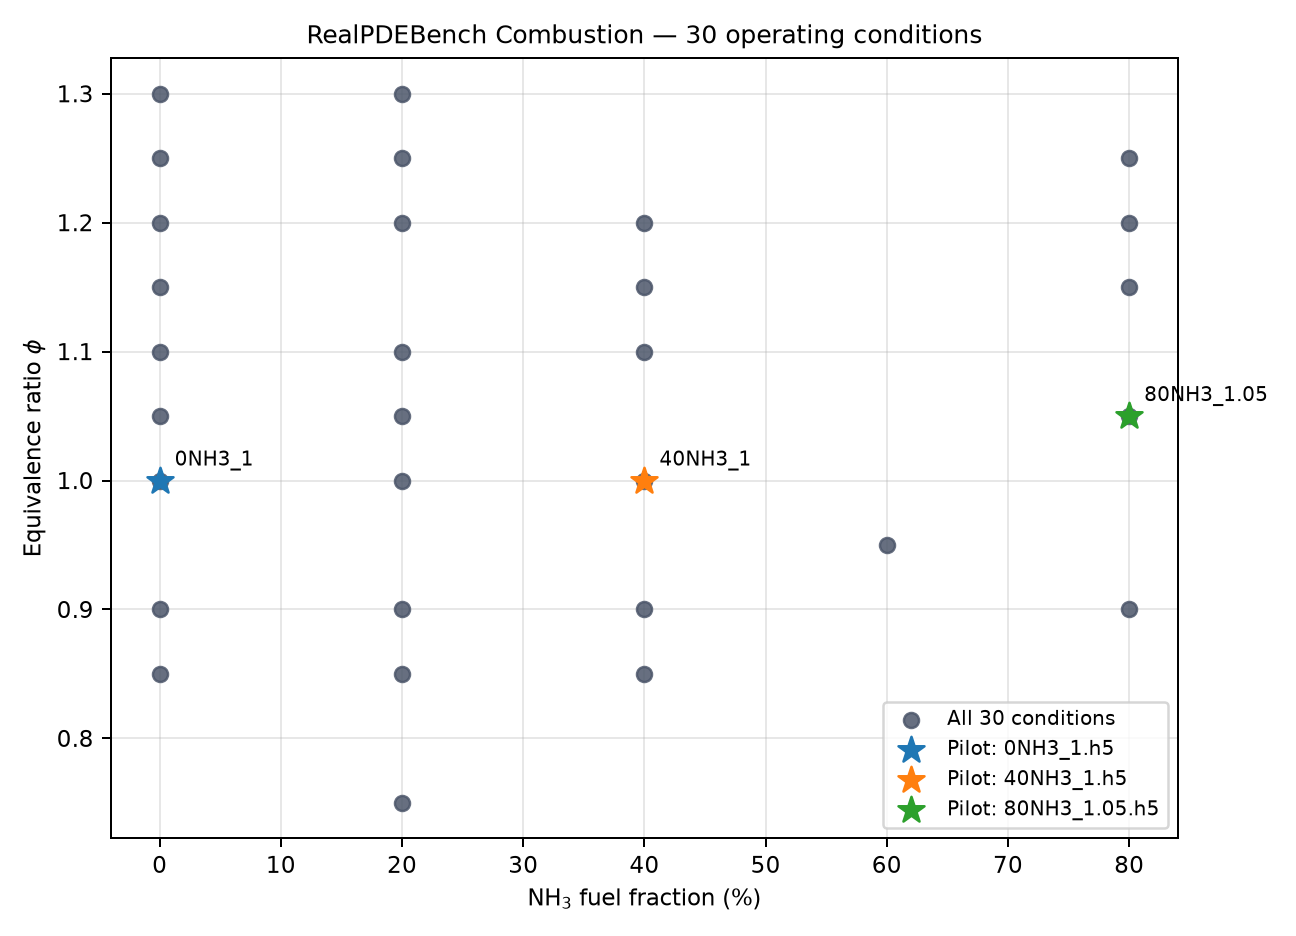
\includegraphics[width=0.74\textwidth]{fig01_parameter_space_30_conditions.png}
    \caption[Operating parameter space of the 30 LES conditions]{Distribution of all 30 numerical LES operating conditions across ammonia fuel fraction ($\text{NH}_3\%$) and equivalence ratio ($\phi$). Highlighted markers indicate the three representative trajectories initially audited in the pilot inspection (\texttt{0NH3\_1.h5}, \texttt{40NH3\_1.h5}, and \texttt{80NH3\_1.05.h5}).}
    \label{fig:data_param_space}
\end{figure}

\subsection{Why Official RealPDEBench Splits Cannot Be Reused Directly}
\label{subsec:data_official_splits}

Inspecting the official index metadata released with \textit{RealPDEBench} (\texttt{train\_\allowbreak{}index\_\allowbreak{}numerical.json}, \texttt{val\_\allowbreak{}index\_\allowbreak{}numerical.json}, and \texttt{test\_\allowbreak{}index\_\allowbreak{}numerical.json}) revealed a structural mismatch with our diagnostic task. In the official benchmark release:
\begin{itemize}
    \item All $30$ numerical conditions ($58{,}860$ temporal windows) are pooled into \texttt{train\_\allowbreak{}index\_\allowbreak{}numerical.json} (\texttt{remain\_\allowbreak{}params\_\allowbreak{}numerical.json} contains 30/30 trajectories), while \texttt{val\_\allowbreak{}index\_\allowbreak{}numerical.json}, \texttt{test\_\allowbreak{}index\_\allowbreak{}numerical.json}, \texttt{in\_\allowbreak{}dist\_\allowbreak{}test\_\allowbreak{}params}, and \texttt{out\_\allowbreak{}dist\_\allowbreak{}test\_\allowbreak{}params} are empty (\texttt{[]} or \texttt{\{\}}). This design reflects \textit{RealPDEBench}'s primary goal: pretraining autoregressive temporal forecasting models ($20 \rightarrow 20$ frames) on half-resolution numerical fields (\texttt{sub\_s = 2}, $64 \times 64$) prior to fine-tuning on experimental line-of-sight $\text{OH}^*$ chemiluminescence sequences ($\sim 3.67\text{ GB}$).
    \item Consequently, reusing the official benchmark indices would test neither cross-variable spatial reconstruction at full $128 \times 128$ resolution (\texttt{sub\_s = 1}) nor generalization to unseen fuel blends and equivalence ratios. This thesis therefore defines its own leakage-free operating-condition split (Section~\ref{sec:data_protocol}).
\end{itemize}

% ==============================================================================
\section{Geometric Orientation, Physical Channels, and Data Quality Audit}
\label{sec:data_geometry}
% ==============================================================================

\subsection{2D Diametral Slice Geometry and Channel Mapping}
\label{subsec:data_geom_channels}

Each Arrow shard stores one complete trajectory at full planar resolution $128 \times 128$ over $2001$ exported snapshots with uniform nominal sampling interval $\Delta t = 2.5 \times 10^{-4}\text{ s}$ ($4000\text{ Hz}$, covering $0.5\text{ s}$ physical duration per trajectory, within absolute simulation windows $t \in [1.5, 2.0]\text{ s}$, $[1.7, 2.2]\text{ s}$, $[3.5, 4.0]\text{ s}$, or $[3.8, 4.3]\text{ s}$). The spatial coordinates are stored as one-dimensional \texttt{float64} arrays of length $128$:
\begin{align}
    x &\in [-0.03691,\; +0.03689]\text{ m} \quad (\text{array axis 1 / columns},\; \Delta x \approx 5.81 \times 10^{-4}\text{ m}), \\
    y &\in [0.06285,\; 0.15913]\text{ m} \quad (\text{array axis 0 / rows},\; \Delta y \approx 7.58 \times 10^{-4}\text{ m}),
\end{align}
spanning a physical observation window of approximately $73.8\text{ mm} \times 96.3\text{ mm}$ located downstream of the burner injector nozzle.

\begin{figure}[H]
    \centering
    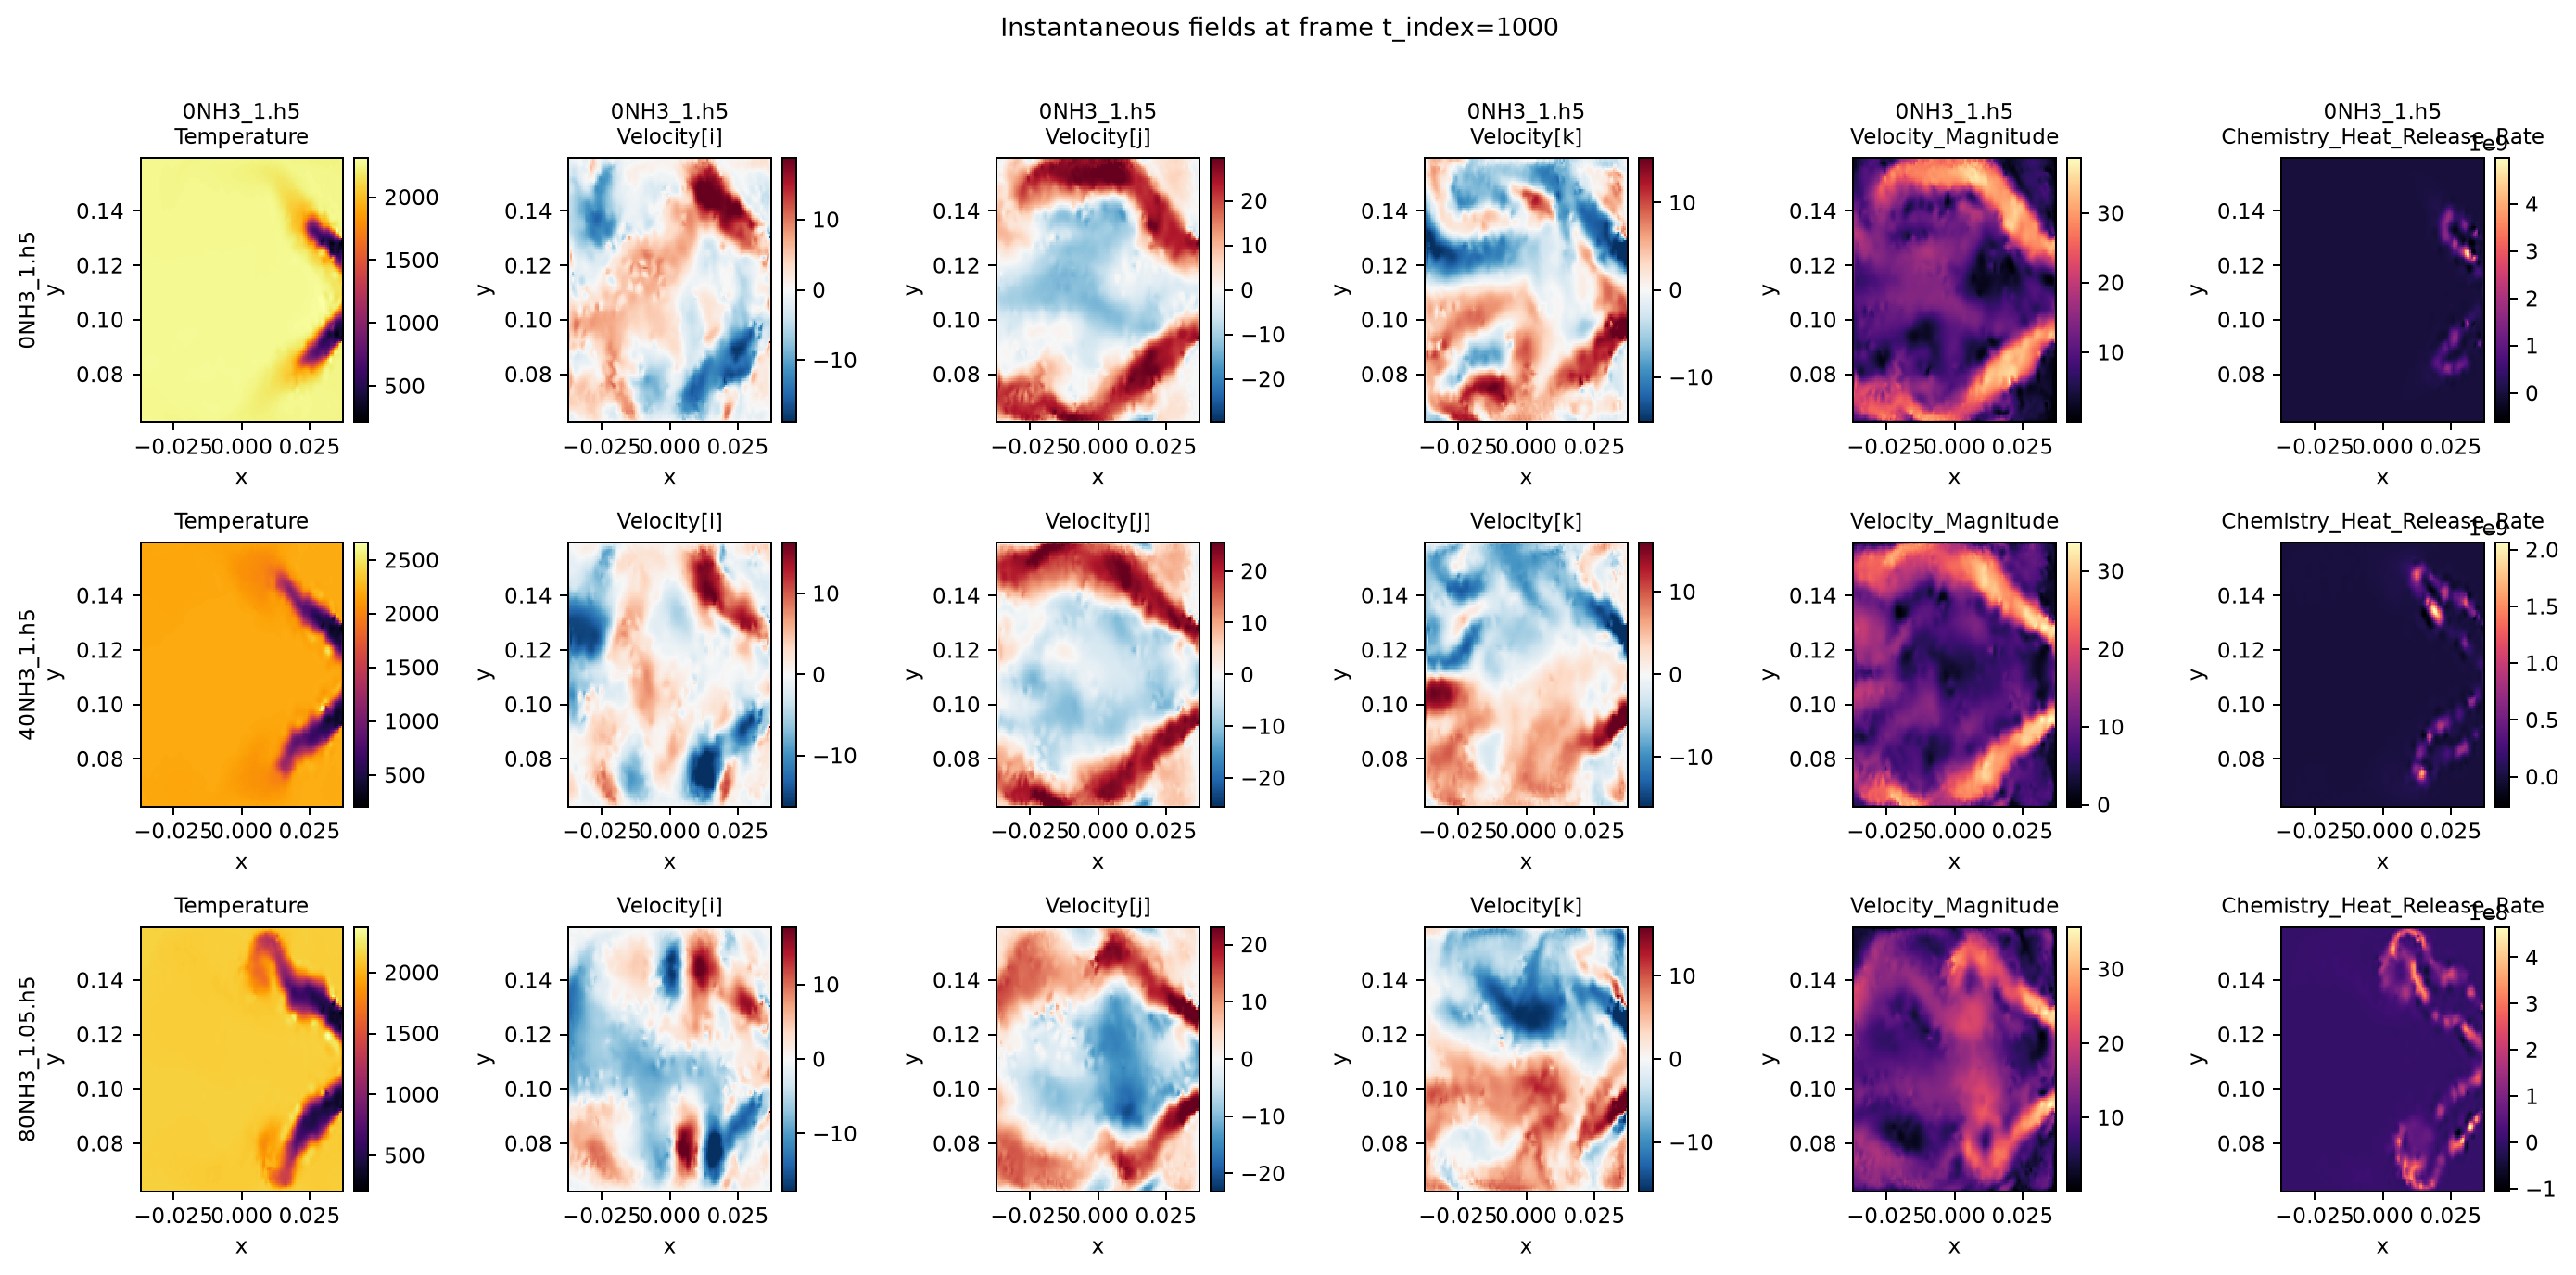
\includegraphics[width=\textwidth]{fig02_pilot_instantaneous_fields.png}
    \caption[Instantaneous physical fields across three representative fuel blends]{Instantaneous LES fields ($T$, $v_i$, $v_j$, $v_k$, exported $|\mathbf{U}|$, and chemical heat release rate) across three pilot operating conditions ($0\%$, $40\%$, and $80\%\text{ NH}_3$ near stoichiometry). Cold reactant jets enter from the right boundary ($x_{\max} \approx +36.9\text{ mm}$) and diverge in a V-shape toward the left, framing the central Inner Recirculation Zone.}
    \label{fig:data_instantaneous}
\end{figure}

\begin{figure}[H]
    \centering
    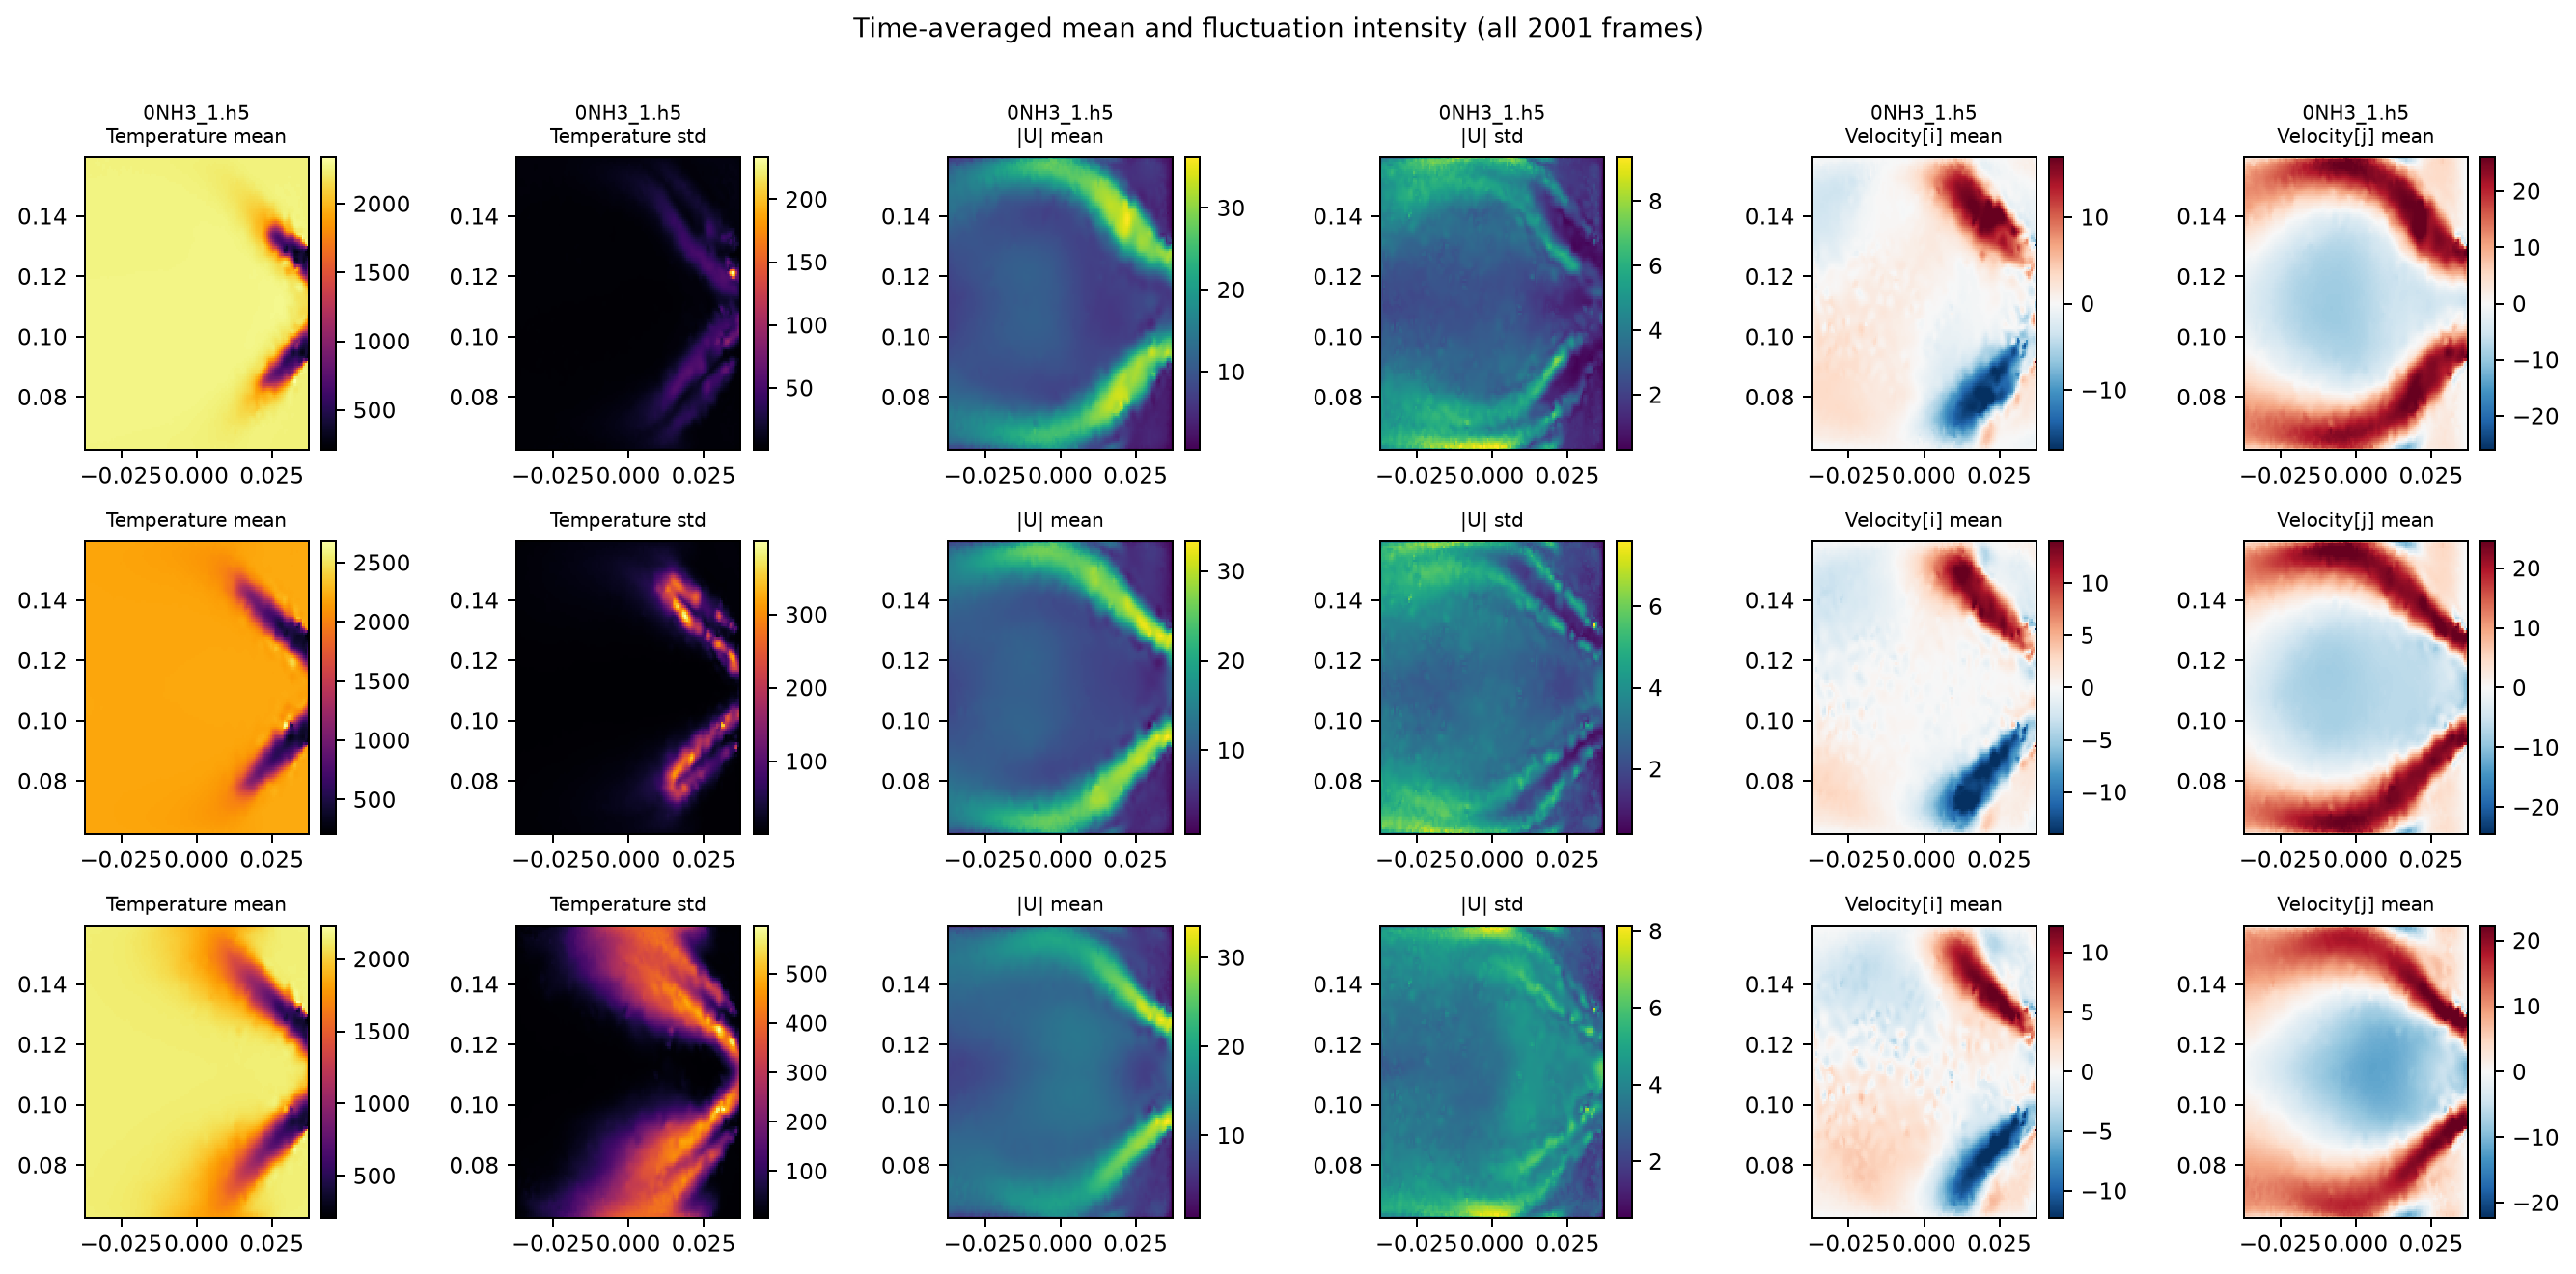
\includegraphics[width=\textwidth]{fig03_pilot_mean_and_std_fields.png}
    \caption[Time-averaged mean and standard deviation of temperature across pilot blends]{Time-averaged mean temperature $\bar{T}$ and temporal standard deviation $\sigma_T$ across the three pilot blends. Peak temperature fluctuations ($\sigma_T \approx 300\text{--}500\text{ K}$) concentrate sharply along the V-shaped shear layers bordering the cold jets, while the interior burnt core remains comparatively uniform.}
    \label{fig:data_mean_std}
\end{figure}

Visual and kinematic inspection of Figures~\ref{fig:data_instantaneous} and~\ref{fig:data_mean_std} establishes the exact physical orientation and channel conventions used throughout this thesis (matching \texttt{channels.json}):
\begin{itemize}
    \item \textbf{Burner symmetry axis and inlet orientation:} The planar field is symmetric about the horizontal centerline near \textbf{row 64} ($y \approx 0.111\text{ m}$). Two cold unburnt reactant branches ($T \approx 300\text{--}400\text{ K}$) enter from the \textbf{right boundary} (\texttt{col = 127}, $x \approx +36.9\text{ mm}$) and diverge radially in a V-shape toward the left (\texttt{col = 0}, $x \approx -36.9\text{ mm}$), enclosing the hot central Inner Recirculation Zone (IRZ). The burner nozzle exit lies immediately outside the cropped field to the right ($x > x_{\max}$).
    \item \textbf{Temperature (Ch~10, target $T$):} Planar LES gas temperature in Kelvin, typically $T \approx 1900\text{--}2280\text{ K}$ inside the burnt recirculation core and $250\text{--}400\text{ K}$ in the incoming reactant cores.
    \item \textbf{Velocity components (Ch~11--13) and directional sign convention:}
    \begin{enumerate}
        \item \texttt{Ch 11 (Velocity[i])}: \textbf{In-plane radial/transverse velocity} $v_i$ [m/s], positive ($+$) in the upper V-branch ($\text{row} > 64$, moving toward $+y$) and negative ($-$) in the lower V-branch ($\text{row} < 64$, moving toward $-y$) as the annular swirling jet expands radially outward.
        \item \texttt{Ch 12 (Velocity[j])}: \textbf{Axial velocity} $v_j$ [m/s], strongly positive ($\sim +20\text{--}30\text{ m/s}$) along the two V-jet branches and negative ($\sim -7\text{ to }-15\text{ m/s}$) inside the central IRZ reverse flow. Crucially, relative to the exported Cartesian grid coordinate $x$, positive $v_j$ points \emph{downstream} toward $-x$ (from right to left); accordingly, physical in-plane streamlines in $(x, y)$ coordinates follow $(-v_j, +v_i)$, and spatial derivatives in $(x, y)$ must respect this sign convention.
        \item \texttt{Ch 13 (Velocity[k])}: \textbf{Out-of-plane azimuthal swirl velocity} $v_k$ [m/s] ($\sim \pm 15\text{ m/s}$), exhibiting antisymmetric signs above and below the symmetry axis (\texttt{row 64}).
    \end{enumerate}
\end{itemize}

\subsection{Data Quality, Physical Guardrails, and Timestamp Anomaly Audit}
\label{subsec:data_quality}

Systematic validation across all $30$ shards ($\sim 9.83 \times 10^8$ space--time grid points) verified zero \texttt{NaN} or \texttt{Inf} entries in any tensor, while uncovering four dataset anomalies that govern how the preprocessing pipeline handles the raw arrays:
\begin{enumerate}
    \item \textbf{Artifacts in exported \texttt{Velocity\_Magnitude} (Ch~14):} Comparison between the exported Ch~14 array and the exact Euclidean norm $|\mathbf{u}| = \sqrt{v_i^2 + v_j^2 + v_k^2}$ computed from Ch~11--13 reveals small numerical interpolation artifacts in Ch~14, including unphysical negative magnitudes down to $-8\text{ m/s}$. Our pipeline therefore discards Ch~14 and always recomputes velocity magnitude directly from the orthogonal velocity components.
    \item \textbf{Rare temperature interpolation outliers (Ch~10):} While the bulk temperature field lies strictly within physical combustion bounds ($[250, 2350]\text{ K}$), grid resampling from the unstructured 3D LES mesh onto the $128 \times 128$ Cartesian slice introduces rare isolated undershoots ($T < 0\text{ K}$ in $15/30$ conditions, typically $10\text{--}600$ voxels out of $3.28 \times 10^7$ per condition, i.e., $\ll 0.01\%$, worst $-375\text{ K}$) and overshoots ($T > 2600\text{ K}$ in $24/30$ conditions, $< 0.03\%$ of voxels, up to $3002\text{ K}$). To maintain transparent target continuity, raw Ch~10 temperatures are preserved without silent clipping during baseline benchmarking, while sensitivity to physical clipping is flagged as a protocol check.
    \item \textbf{Separation of planar $\text{OH}$ (Ch~8) and experimental $\text{OH}^*$ (\texttt{observed}):} In \textit{RealPDEBench}, the \texttt{observed} array represents line-of-sight integrated $\text{OH}^*$ chemiluminescence intensity (mapped from numerical fields by the benchmark's surrogate network), whereas Ch~8 (\texttt{Mole\_Fraction\_of\_OH}) is the 2D planar LES species concentration. Neither channel is ever conflated with the other or passed into velocity-to-temperature inputs.
    \item \textbf{Interior timestamp gap and duplicate frame in \texttt{40NH3\_1.2.h5} (shard \texttt{data-00022-of-00030.arrow}):} A fine-grained timeline audit conducted during pipeline hardening established that while the numerical tensor of \texttt{40NH3\_1.2.h5} has shape $(2001, 128, 128, 15)$, its exported time coordinate array \texttt{t} contains only $2000$ entries spanning $[1.5, 2.0]\text{ s}$ with a single interior step doubling ($\Delta t_{1098} \approx 5.0 \times 10^{-4}\text{ s}$ corresponding to deletion of uniform index $1099$) and bitwise-identical field snapshots at indices $1999$ and $2000$. Consequently, single-frame instantaneous reconstruction indexed by snapshot ID remains valid, whereas unverified multi-frame or temporal forecasting evaluation on this shard is explicitly blocked by dataset metadata flags (\texttt{field\_time\_association\_verified = False}).
\end{enumerate}

% ==============================================================================
\section{Thermodynamic Trends, Temporal Autocorrelation, and Kinematic Coupling}
\label{sec:data_coupling}
% ==============================================================================

\subsection{Parametric Trends Across the 30 Operating Conditions}
\label{subsec:data_trends}

Figure~\ref{fig:data_trends} summarizes how key thermal and kinematic quantities vary across the 30 conditions as functions of $\text{NH}_3\%$ and $\phi$:
\begin{itemize}
    \item \textbf{Systematic cooling and deeper cold-jet penetration with ammonia blending:} At matched equivalence ratio $\phi$, domain-mean temperature drops by $185\text{--}225\text{ K}$ from $0\%\text{ NH}_3$ ($\bar{T} = 2000.4\text{--}2186.5\text{ K}$) to $80\%\text{ NH}_3$ ($\bar{T} = 1864.5\text{--}1957.2\text{ K}$), while the mean volume fraction of cold unburnt pockets ($T < 1200\text{ K}$) more than doubles from $3.5\%$ to $8.5\%$. Within each fixed $\text{NH}_3$ band, $\bar{T}$ peaks near $\phi \approx 1.0\text{--}1.05$ and decreases sharply toward both lean ($\phi = 0.75$) and rich ($\phi = 1.25\text{--}1.30$) limits, reflecting lower heat release and chemical dilution. Meanwhile, fully burnt gases ($T > 1800\text{ K}$) occupy $81\%\text{--}96\%$ of the observation window across all 30 conditions.
    \item \textbf{Bulk velocity trends:} Across $28$ of the $30$ conditions, recomputed mean flow speed $\overline{|\mathbf{u}|}$ remains tightly clustered between $10.0$ and $14.9\text{ m/s}$, generally decreasing with increasing $\phi$ within each fuel blend ($r \in [-0.76, -0.99]$, with a slight upward inflection at $\phi = 1.2$ in $20\%\text{ NH}_3$). Two lean pure-methane trajectories (\texttt{0NH3\_0.85} and \texttt{0NH3\_0.90}) exhibit noticeably higher bulk flow speeds ($23.77$ and $17.3\text{ m/s}$, respectively), consistent with inflow mass-flow adjustments used to vary $\phi$ in those operating points.
\end{itemize}

\begin{figure}[H]
    \centering
    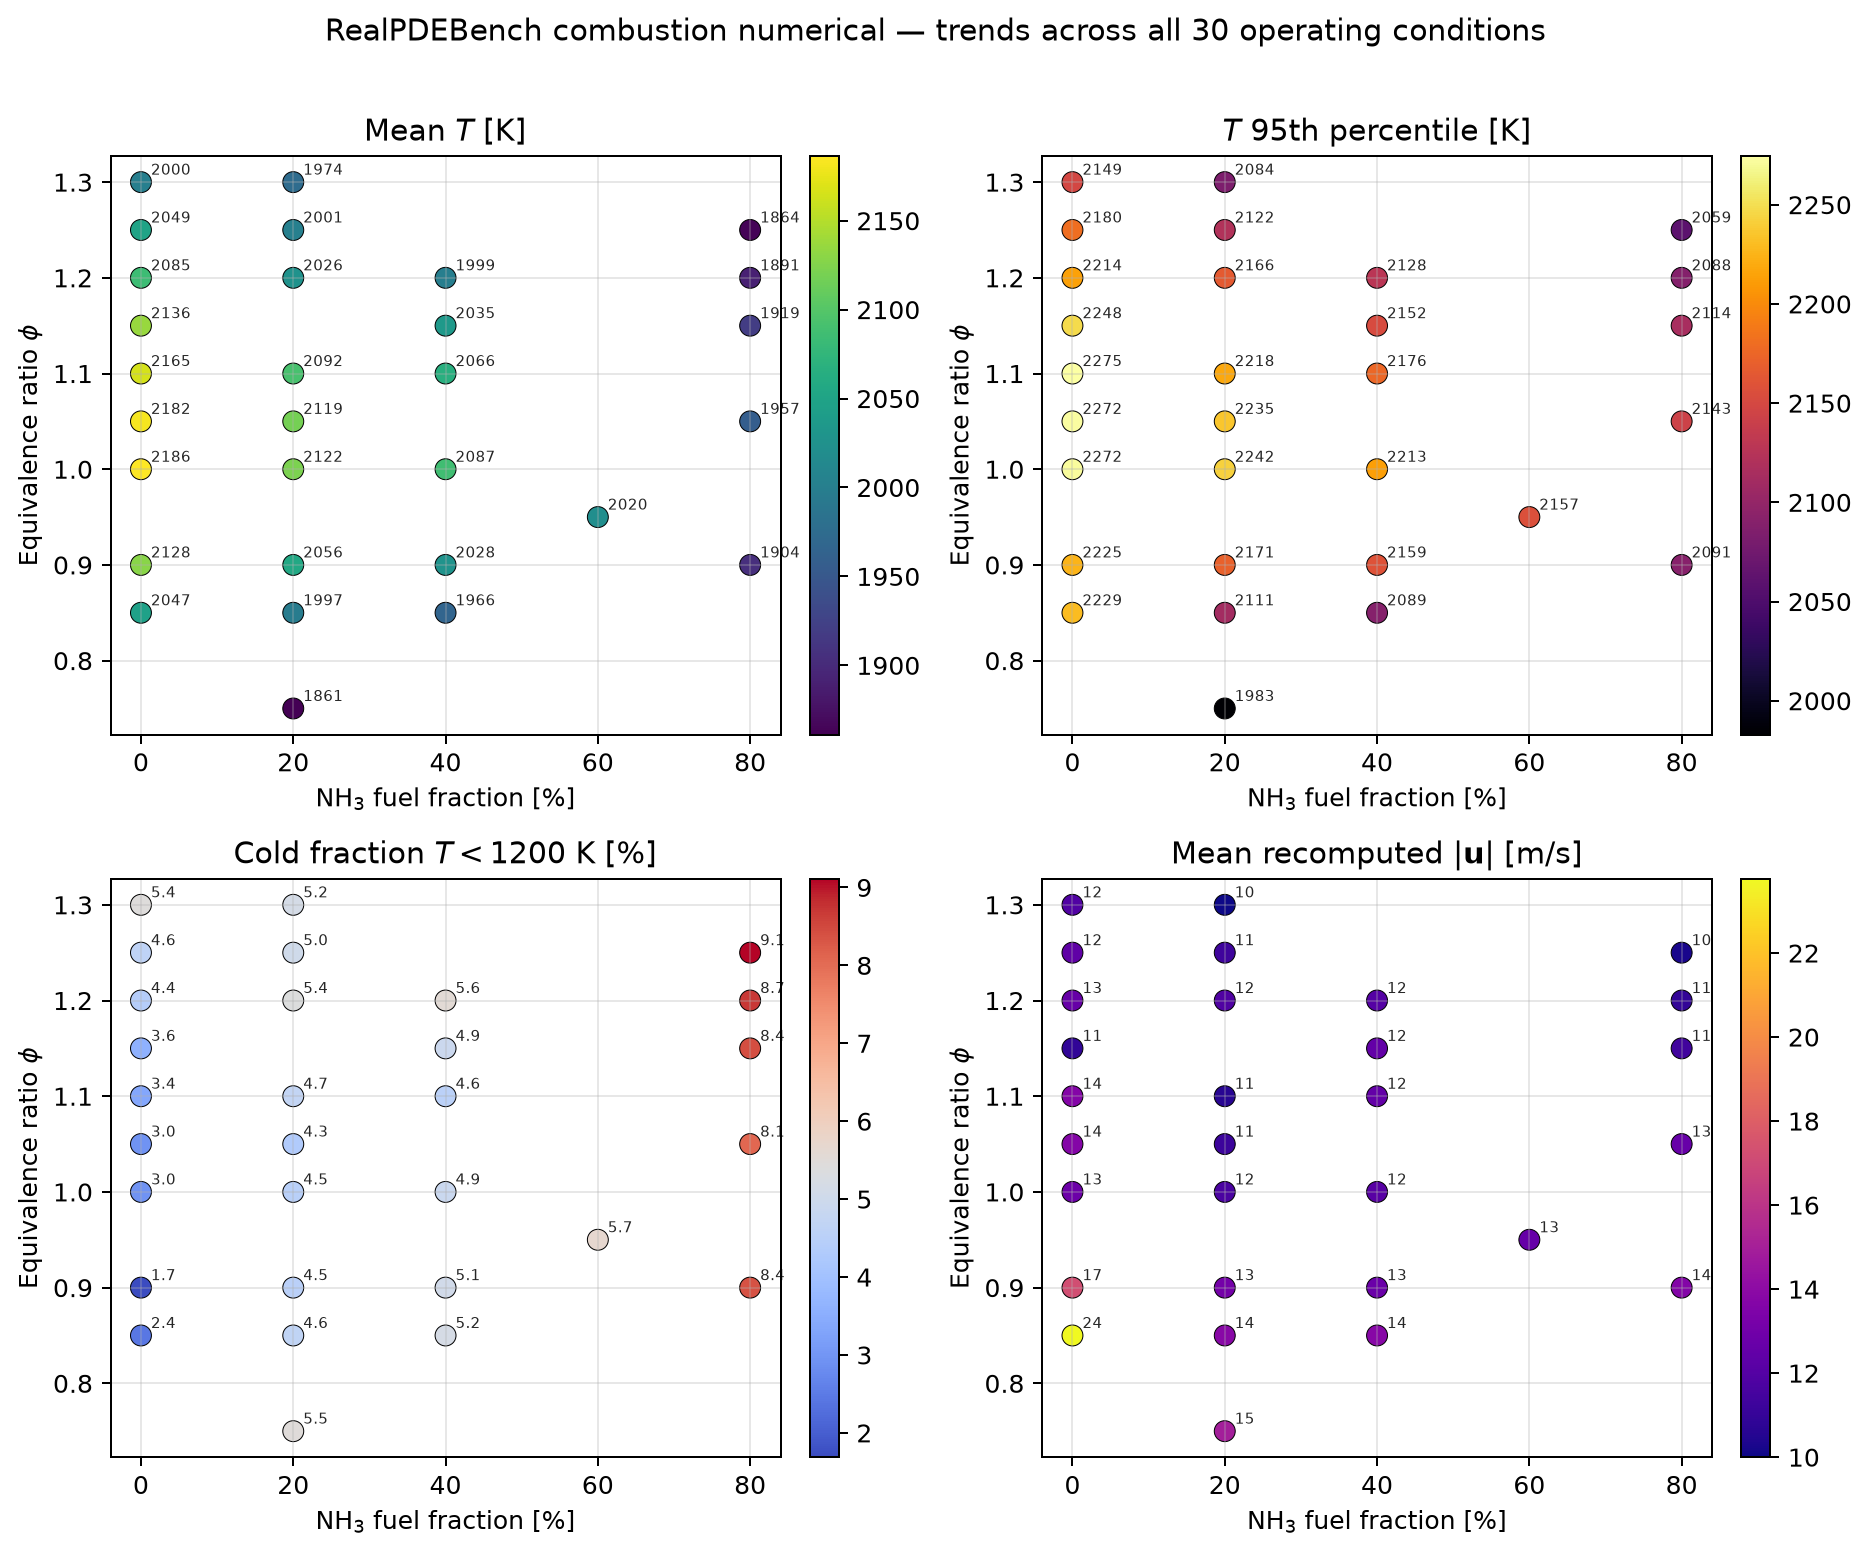
\includegraphics[width=0.96\textwidth]{fig05_all30_temperature_velocity_trends.png}
    \caption[Thermodynamic and kinematic trends across all 30 LES operating conditions]{Trends across all 30 LES operating conditions vs.\ equivalence ratio $\phi$, grouped by $\text{NH}_3\%$ fraction: domain-mean temperature $\bar{T}$, 95th-percentile temperature $T_{p95}$, cold reactant fraction ($T < 1200\text{ K}$), and recomputed mean velocity magnitude $\overline{|\mathbf{u}|}$.}
    \label{fig:data_trends}
\end{figure}

\subsection{Temperature Histograms and Flame-Brush Temporal Autocorrelation}
\label{subsec:data_autocorr}

Figure~\ref{fig:data_hist_autocorr} examines the marginal temperature distributions and temporal decorrelation timescales on the three pilot trajectories. Across all blends, the temperature histogram is strongly bimodal and burnt-dominated: a sharp peak centered around $2050\text{--}2250\text{ K}$ accounts for roughly $90\%$ of space--time voxels, accompanied by a long low-temperature shoulder ($300\text{--}1800\text{ K}$) corresponding to the cold annular jets and reaction mixing layer whose weight expands systematically with $\text{NH}_3\%$. Along the transverse midline cut (Figure~\ref{fig:data_hist_autocorr}, panel a2), the radial temperature profile shows two symmetric cold dips near rows $\sim 40$ and $\sim 88$ corresponding to the upper and lower branches of the annular jet.

\begin{figure}[H]
    \centering
    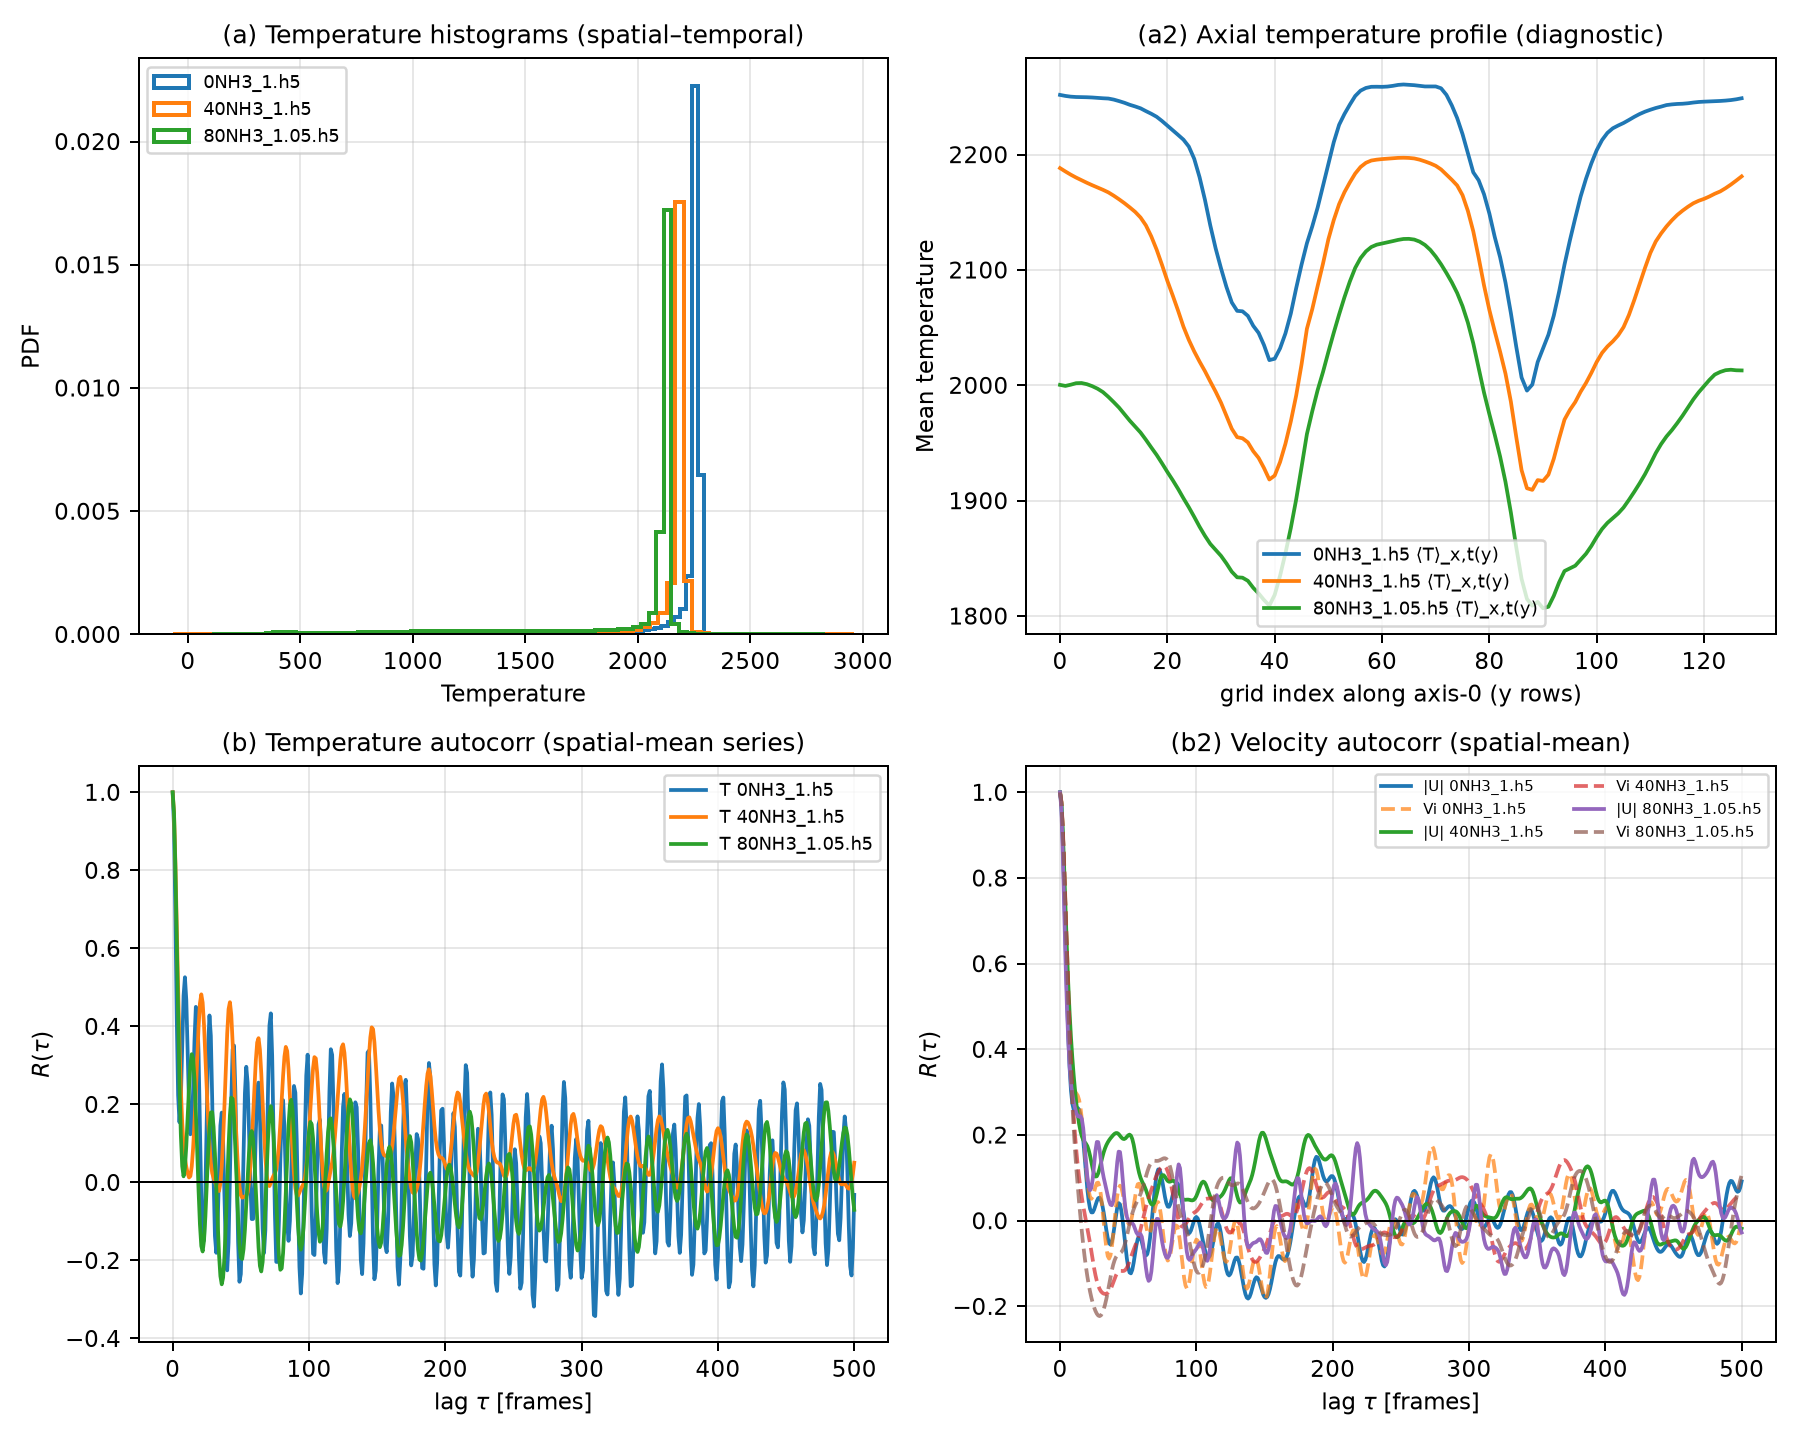
\includegraphics[width=\textwidth]{fig04_temperature_histograms_and_autocorr.png}
    \caption[Temperature distributions and temporal autocorrelation timescales]{(a1--a2)~Temperature distributions and mean radial profiles across rows ($y$) showing symmetric cold jet dips near rows $40$ and $88$. (b1--b2)~Temporal autocorrelation functions $R(\Delta t)$ of domain-mean temperature versus high-variance flame-brush points: local flame-front fluctuations remain correlated over $50\text{--}100+$ frames ($\tau_c \approx 14\text{ ms}$).}
    \label{fig:data_hist_autocorr}
\end{figure}

Crucially, panel~(b) of Figure~\ref{fig:data_hist_autocorr} reveals a two-scale temporal decorrelation structure. While the domain-averaged temperature decays over $O(10\text{--}20)$ frames ($\sim 2.5\text{--}5\text{ ms}$), individual spatial locations inside the high-variance flame brush retain significant temporal correlation across \textbf{$50\text{--}100+$ consecutive frames} ($\tau_c \approx 14\text{ ms}$ at $4000\text{ Hz}$). Splitting frames randomly within a single trajectory would therefore place nearly identical flame snapshots in both training and test sets, inflating apparent generalization through temporal memorization.

\subsection{Kinematic--Thermal Coupling and Cross-Condition Ambiguity}
\label{subsec:data_kinematic_check}

Before fitting any reconstruction model, we quantified the physical coupling between velocity features (and spatial velocity derivatives) and temperature across the 20 training trajectories (\texttt{Check 1}, Table~\ref{tab:data_check1} and Figure~\ref{fig:data_check1}):

\begin{table}[H]
\centering
\caption[Pointwise kinematic--thermal correlations with temperature]{Pointwise correlations between velocity / kinematic gradient features and temperature $T$ across the 20 training conditions (\texttt{Check 1}), comparing pooled multi-condition statistics (Pearson $r$, Spearman $\rho$, and mutual information MI) against within-condition Pearson $r$ (mean $\pm$ std across the 20 trajectories).}
\label{tab:data_check1}
\small
\resizebox{\textwidth}{!}{%
\begin{tabular}{lrrrr}
\toprule
\textbf{Feature} & \textbf{Pooled Pearson $r$} & \textbf{Pooled Spearman $\rho$} & \textbf{Pooled MI} & \textbf{Within-Cond. Pearson $r$} \\
\midrule
Velocity magnitude $|\mathbf{u}|$ & $-0.3788$ & $-0.2798$ & $0.1169$ & $-0.474 \pm 0.114$ \\
Axial velocity $v_j$ & $-0.3196$ & $-0.2057$ & $0.1282$ & $-0.384 \pm 0.120$ \\
Strain-rate magnitude $\|S_{\text{2D}}\|$ & $-0.1231$ & $-0.1302$ & $0.0224$ & $-0.250 \pm 0.091$ \\
Out-of-plane vorticity $|\omega_z|$ & $-0.0643$ & $-0.0639$ & $0.0175$ & $-0.198 \pm 0.058$ \\
Planar dilatation $\nabla_{\text{2D}}\cdot\mathbf{u}$ & $-0.0204$ & $+0.0092$ & $0.0125$ & $-0.025 \pm 0.060$ \\
Azimuthal swirl $v_k$ & $+0.0103$ & $+0.0173$ & $0.0778$ & $+0.004 \pm 0.014$ \\
Radial velocity $v_i$ & $+0.0065$ & $+0.0141$ & $0.0706$ & $+0.003 \pm 0.024$ \\
\bottomrule
\end{tabular}%
}
\end{table}

\begin{figure}[H]
    \centering
    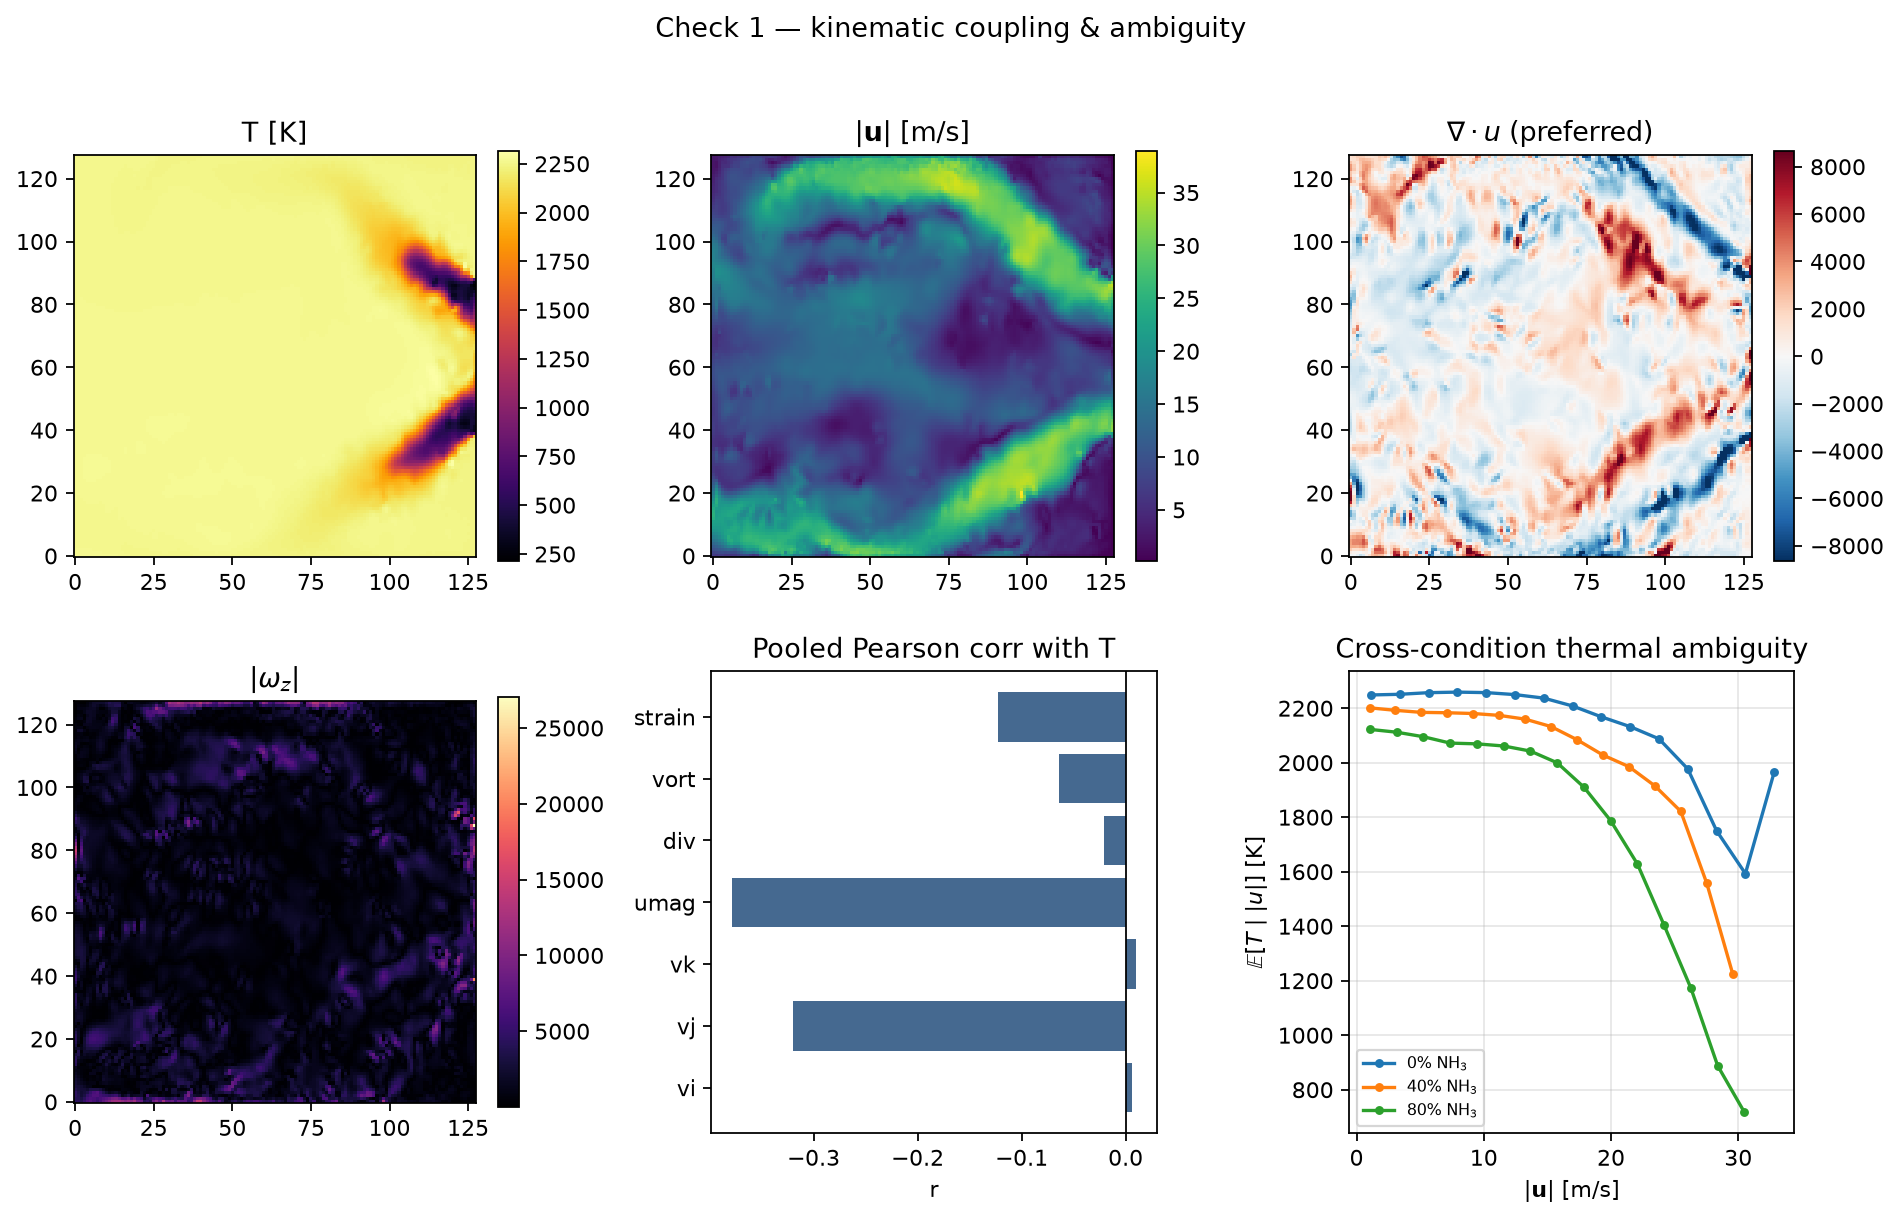
\includegraphics[width=\textwidth]{fig07_kinematic_coupling_and_ambiguity.png}
    \caption[Kinematic--thermal coupling and cross-condition thermal ambiguity]{Physical feasibility analysis (\texttt{Check 1}): instantaneous $T$, $|\mathbf{u}|$, planar dilatation $\nabla_{\text{2D}}\cdot\mathbf{u}$, and vorticity $|\omega_z|$ on a stoichiometric methane snapshot (\texttt{0NH3\_1.h5}), alongside pooled Pearson correlations with $T$ and conditional expectation curves $\mathbb{E}[T \mid |\mathbf{u}|]$ across $0\%$, $40\%$, and $80\%\text{ NH}_3$ blends.}
    \label{fig:data_check1}
\end{figure}

Table~\ref{tab:data_check1} and Figure~\ref{fig:data_check1} establish three essential physical properties of the inverse problem:
\begin{enumerate}
    \item \textbf{Within-condition spatial localization:} Within any fixed operating condition, velocity magnitude $|\mathbf{u}|$ ($r = -0.474 \pm 0.114$) and axial velocity $v_j$ ($r = -0.384 \pm 0.120$) correlate strongly and negatively with temperature because high-momentum V-jets transport cold reactants whereas low-speed recirculation cores hold hot burnt gas. Notice that $v_i$ and $v_k$ show near-zero linear correlation with $T$ solely because they are antisymmetric about the burner axis (\texttt{row 64}) while $T$ is symmetric---yet they carry significant mutual information ($\text{MI} = 0.071\text{--}0.078$).
    \item \textbf{Cross-condition thermodynamic confounding:} Pooling samples across all 20 conditions weakens the linear correlation ($|\mathbf{u}|$: $-0.474 \rightarrow -0.379$), and the conditional expectation curves $\mathbb{E}[T \mid |\mathbf{u}|]$ (Figure~\ref{fig:data_check1}, bottom right) separate vertically by \textbf{$200\text{--}360\text{ K}$} between $0\%$, $40\%$, and $80\%\text{ NH}_3$ at identical local flow speeds (e.g., $\sim 2150\text{ K}$ vs.\ $\sim 1800\text{ K}$ at $|\mathbf{u}| = 20\text{ m/s}$). Local velocity observations alone are therefore thermodynamically ambiguous without knowledge of $\mathbf{p} = (\text{NH}_3\%, \phi)$ or sparse temperature anchors.
    \item \textbf{Thin-sheet localization of planar dilatation:} Pointwise planar divergence $\nabla_{\text{2D}}\cdot\mathbf{u}$ has near-zero correlation with bulk temperature $T$ ($r = -0.0204$), whereas on the representative \texttt{0NH3\_1.h5} snapshot the magnitude $|\nabla_{\text{2D}}\cdot\mathbf{u}|$ correlates positively with the flame-front temperature gradient $|\nabla T|$ ($r = +0.2368$). Consistent with the low-Mach physics in Section~\ref{sec:bg_pinns}, dilatation is concentrated along the thin reaction sheet (and polluted by unclosed $\partial_z v_k$ out-of-plane swirl divergence) rather than varying proportionally with bulk $T$.
\end{enumerate}

% ==============================================================================
\section{Locked Operating-Condition Splits and Decomposed Evaluation Protocol}
\label{sec:data_protocol}
% ==============================================================================

\subsection{Condition-Level Partition and Temporal Protocol}
\label{subsec:data_splits}

To eliminate trajectory-level leakage across the $50\text{--}100$ frame correlation horizon, all $30$ operating conditions are partitioned strictly at the trajectory level into four disjoint splits (\texttt{configs/splits/splits\_interp\_extrap.yaml}, Figure~\ref{fig:data_splits}):

\begin{table}[H]
\centering
\caption[Locked operating-condition partition across the 30 LES trajectories]{Locked operating-condition split across the 30 LES simulations ($20+3+3+4 = 30$, zero overlap). Within each training condition, fit and seen-evaluation temporal indices are separated by a $120$-frame ($\ge 2\tau_c$) buffer.}
\label{tab:data_splits}
\small
\resizebox{\textwidth}{!}{%
\begin{tabular}{lrp{6.8cm}p{4.3cm}}
\toprule
\textbf{Split} & \textbf{\# Cond.} & \textbf{Assigned Operating Conditions (\texttt{sim\_id})} & \textbf{Scientific Role} \\
\midrule
\texttt{train} & 20 & \texttt{0NH3}: $0.85, 0.90, 1.00, 1.10, 1.15, 1.20, 1.25$; \newline \texttt{20NH3}: $0.85, 0.90, 1.05, 1.20, 1.25$; \newline \texttt{40NH3}: $0.85, 1.00, 1.10, 1.20$; \newline \texttt{80NH3}: $0.90, 1.05, 1.15, 1.20$ & Model fitting (\texttt{train\_fit}: frames $0\text{:}1480\text{:}40$, 38/traj = 760) and seen diagnostics (\texttt{seen\_train\_eval}: frames $1600\text{:}2000\text{:}40$, 11/traj = 220) \\
\midrule
\texttt{val} & 3 & \texttt{0NH3\_1.05}, \texttt{20NH3\_1.10}, \texttt{40NH3\_0.90} & Architecture and hyperparameter selection (frames $0\text{:}2000\text{:}50$, 41/traj = 123) \\
\midrule
\texttt{test\_interp} & 3 & \texttt{20NH3\_1.00}, \texttt{40NH3\_1.15}, \texttt{60NH3\_0.95} & Held-out transfer strictly inside the $(\text{NH}_3\%, \phi)$ training hull (including unseen $60\%\text{ NH}_3$ blend; 41/traj = 123) \\
\midrule
\texttt{test\_extrap} & 4 & \texttt{20NH3\_0.75} (leanest), \texttt{0NH3\_1.30}, \texttt{20NH3\_1.30} (richest), \texttt{80NH3\_1.25} (high-$\text{NH}_3$ rich corner) & Held-out boundary and out-of-range generalization (41/traj = 164) \\
\bottomrule
\end{tabular}%
}
\end{table}

\begin{figure}[H]
    \centering
    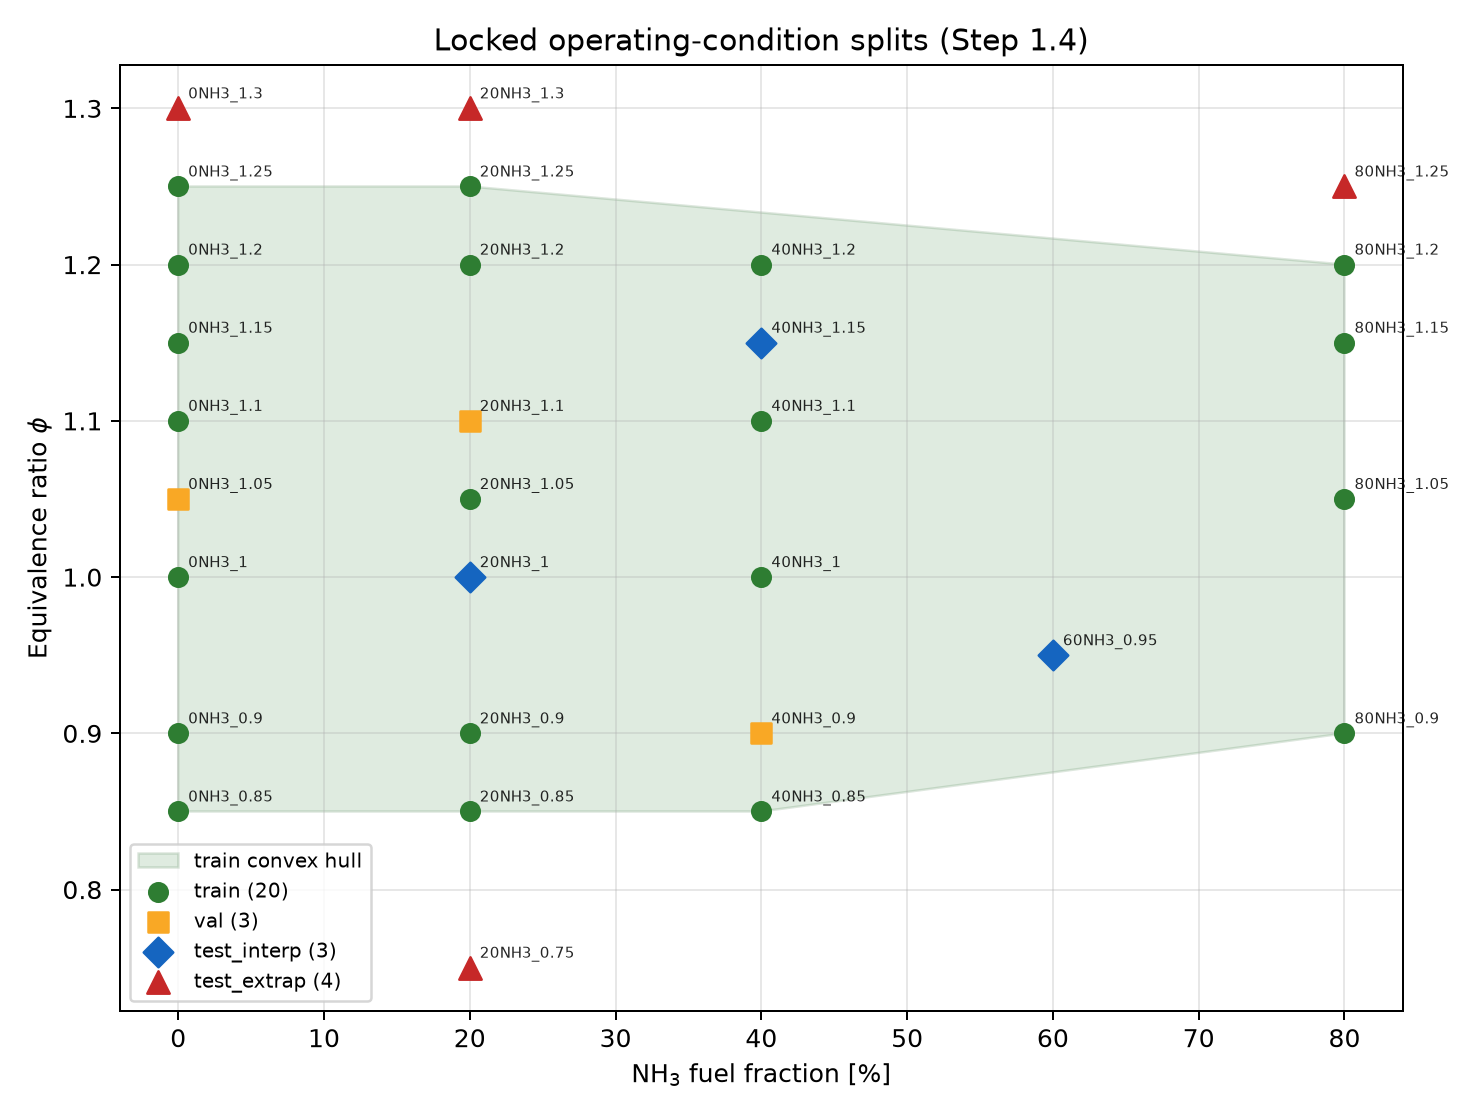
\includegraphics[width=0.66\textwidth]{fig06_locked_operating_condition_splits.png}
    \caption[Locked operating-condition splits across the parameter space]{Locked partition of the 30 operating conditions into \texttt{train} (20), \texttt{val} (3), \texttt{test\_interp} (3), and \texttt{test\_extrap} (4), with the shaded polygon indicating the training convex hull.}
    \label{fig:data_splits}
\end{figure}

As detailed in Table~\ref{tab:data_splits}, all held-out conditions (\texttt{val}, \texttt{test\_interp}, \texttt{test\_extrap}) remain strictly disjoint from training. Inside the 20 training trajectories, models are fit exclusively on the first 75\% of each simulation (\texttt{train\_fit}: frame indices $0\text{--}1480$ strided by $40$, yielding $760$ snapshots), whereas seen-condition diagnostics are evaluated on the final 20\% (\texttt{seen\_train\_eval}: frame indices $1600\text{--}2000$ strided by $40$, yielding $220$ snapshots) after a $120$-frame ($30\text{ ms} \ge 2\tau_c$) separation buffer.

\subsection{Fit-Only Normalization Statistics}
\label{subsec:data_normalization}

All field z-score normalizations ($\tilde{q} = (q - \mu_q) / \sigma_q$) and operating-parameter scalings are computed exclusively on training data without touching \texttt{val} or \texttt{test} trajectories. Table~\ref{tab:data_norm_stats} compares the initial Month-1 training-condition statistics (all $2001$ frames of the $20$ training trajectories) against the tightened Month-2 \texttt{train\_fit}-only statistics restricted strictly to the $760$ fit frames ($0\text{--}1480$): excluding the seen-evaluation block alters $\mu_T$ and $\sigma_T$ by less than $0.3\text{ K}$ ($0.05\%$) while guaranteeing zero temporal leakage into normalization constants.

\begin{table}[H]
\centering
\caption[Training-only normalization statistics]{Training-only normalization statistics (Welford online unclipped mean and standard deviation) across the 20 training conditions, comparing all-frame training statistics (\texttt{train\_\allowbreak{}norm\_\allowbreak{}stats.json}) against the strict \texttt{train\_fit}-only statistics (\texttt{train\_\allowbreak{}norm\_\allowbreak{}stats\_\allowbreak{}month2\_\allowbreak{}fit.json}, 760 snapshots).}
\label{tab:data_norm_stats}
\small
\resizebox{\textwidth}{!}{%
\begin{tabular}{lrrrr}
\toprule
\textbf{Variable} & \multicolumn{2}{c}{\textbf{Month-1 All-Train Frames (2001/traj)}} & \multicolumn{2}{c}{\textbf{Month-2 Strict \texttt{train\_fit} (38/traj)}} \\
\cmidrule(lr){2-3} \cmidrule(lr){4-5}
 & \textbf{Mean $\mu$} & \textbf{Std $\sigma$} & \textbf{Mean $\mu$} & \textbf{Std $\sigma$} \\
\midrule
Temperature $T$ [K] (Ch~10) & $2039.28$ & $331.58$ & $2039.51$ & $331.74$ \\
Radial velocity $v_i$ [m/s] (Ch~11) & $-0.070$ & $5.689$ & $-0.060$ & $5.674$ \\
Axial velocity $v_j$ [m/s] (Ch~12) & $4.316$ & $11.894$ & $4.272$ & $11.910$ \\
Azimuthal swirl $v_k$ [m/s] (Ch~13) & $0.002$ & $7.047$ & \multicolumn{2}{c}{\textit{(ablation channel)}} \\
Operating parameter $\text{NH}_3\%$ & $0.290$ & $0.293$ & $0.290$ & $0.301$ \\
Operating parameter $\phi$ & $1.0575$ & $0.1390$ & $1.0575$ & $0.1426$ \\
\bottomrule
\end{tabular}%
}
\end{table}

\subsection{Standardized Sparse Observation Layouts}
\label{subsec:data_masks}

To decouple sensor spatial geometry from operating-condition transfer, observation masks are generated deterministically on the $128 \times 128$ ($16{,}384$-pixel) grid using \texttt{zlib.crc32} seeds (\texttt{configs/masks/observation\_layouts.yaml}). In \textbf{Track 1 (\texttt{temperature\_free})}, velocity measurements are observed at a subset of pixels under either random sparse PIV sampling ($0.5\% \approx 82$ vectors, $1\% \approx 164$, $2\% \approx 328$, $5\% \approx 819$, $10\% \approx 1638$, and $20\% \approx 3277$ vectors, with $5\%$ serving as the primary sparse benchmark), structured linear rakes (e.g., axial centerline cut at \texttt{row 64} or radial cut at \texttt{col 64}), or localized rectangular optical occlusions ($40 \times 40$ block over the shear layer or $32 \times 32$ block over the IRZ core). In \textbf{Track 2 (\texttt{temperature\_assisted})}, the same velocity mask is augmented with $K \in \{1, 4, 9, 16, 32\}$ nested point temperature probes generated via a fixed spatial permutation so that probe sets obey exact nesting ($1 \subset 4 \subset 9 \subset 16 \subset 32$). Unobserved locations are never passed as physical zeros; models consume either sparse coordinate--value tokens or explicit value-plus-mask channels.

\subsection{Decomposed Error Metrics and Thermal Regions}
\label{subsec:data_metrics}

In a burnt-dominated combustor where $81\%\text{--}96\%$ of pixels exceed $1800\text{ K}$ while steep reaction-zone gradients occupy roughly $10\%$ of the domain, reporting only domain-averaged RMSE obscures whether an error originates from a uniform thermodynamic level shift across mixtures or from mislocating the wrinkled instantaneous flame front. For every reconstructed snapshot $\hat{T}$ against ground truth $T$ over the $N = 16{,}384$ grid pixels, we therefore apply the exact variance decomposition:
\begin{equation}
    \text{RMSE}^2 = \frac{1}{N}\sum_{n=1}^{N} (\hat{T}_n - T_n)^2 = \underbrace{\left(\langle\hat{T}\rangle - \langle T\rangle\right)^2}_{\text{Bias}^2} + \underbrace{\frac{1}{N}\sum_{n=1}^{N} \left[(\hat{T}_n - \langle\hat{T}\rangle) - (T_n - \langle T\rangle)\right]^2}_{\text{Centered-RMSE}^2},
    \label{eq:data_rmse_decomp}
\end{equation}
where $\text{Bias} = \langle\hat{T} - T\rangle$ measures the signed mean thermal level shift on that frame, $|\text{Bias}|$ measures its frame-wise magnitude (preventing cancellation of positive and negative level errors across conditions), and $\text{Centered-RMSE}$ isolates the zero-mean spatial pattern and flame-shape error. Metrics are computed per frame, averaged per condition (\texttt{sim\_id}), and reported both per condition and as unweighted split means.

Finally, to localize errors to the physical regimes relevant to combustor diagnostics, three disjoint or nested spatial masks are evaluated per snapshot (\texttt{configs/splits/evaluation\_protocol.yaml}):
\begin{itemize}
    \item \textbf{High-temperature core ($\Omega_{\text{high}}: T \ge 2100\text{ K}$)} and \textbf{Peak thermal zone ($\Omega_{\text{peak}}: T \ge 2200\text{ K}$)}, evaluated via conditional RMSE/MAE and mask overlap (Intersection-over-Union, IoU).
    \item \textbf{Cold-jet and reaction mixing region ($\Omega_{\text{jet}}: T < 1800\text{ K}$)}, isolating the high-gradient flame front and unburnt V-jets.
\end{itemize}
Across the locked splits, $\Omega_{\text{high}}$ covers $60.2\%$ of voxels in \texttt{train}, $85.9\%$ in \texttt{val}, and $82.4\%$ in \texttt{test\_interp}, but drops to only $11.6\%$ in the cooler extreme conditions of \texttt{test\_extrap} (dropping below $1.1\%$ in three of the four extrapolation conditions, where $\Omega_{\text{peak}}$ falls to $0.1\%$). Meanwhile, $\Omega_{\text{jet}}$ spans $9.2\%$ (\texttt{train}), $6.9\%$ (\texttt{val}), $8.8\%$ (\texttt{test\_interp}), and $12.2\%$ (\texttt{test\_extrap}). Fixed-threshold IoU at $2100\text{ K}$ is therefore strongly governed by mean level accuracy on \texttt{test\_extrap}, reinforcing the primary use of $\text{Centered-RMSE}$ and conditional $\Omega_{\text{jet}}$ RMSE for evaluating instantaneous flame-front structure across regimes.
